\documentclass[12pt,twoside]{report}
\usepackage[a4paper,width=15cm,top=2cm,bottom=2cm,bindingoffset=14mm]{geometry}

\usepackage[utf8]{vietnam}
\usepackage{lipsum}
%\usepackage{showframe}

\usepackage{scrextend}
\changefontsizes[15pt]{13pt}

\usepackage{mathptmx}	% same Time New Roma

\usepackage{bkthesis}
\crname{TIỂU LUẬN}
\ctname{MÔN HỌC: KINH TẾ CÁC NGÀNH SẢN XUẤT KINH DOANH}
\csSupervise{PGS. TS. Phạm Văn ABC}

\usepackage[nottoc]{tocbibind}
%--------------------------------------




\usepackage{amsmath} % needed for command eqref
\usepackage{amssymb} % needed for math fonts
\usepackage[colorlinks=true,breaklinks]{hyperref}

\usepackage{xcolor}
\definecolor{c1}{rgb}{0,0,1} % blue
\definecolor{c2}{rgb}{0,0.3,0.9} % light blue
\definecolor{c3}{rgb}{0.3,0,0.9} % red blue
\hypersetup{
    linkcolor={c1}, % internal links
    citecolor={c2}, % citations
    urlcolor={c3} % external links/urls
}
\usepackage{graphicx}





%--------------------------------------
\usepackage{fancyhdr}
\fancyhf{}
\renewcommand{\chaptermark}[1]{\markboth{#1}{}}
\renewcommand{\sectionmark}[1]{\markright{\thesection\ #1}}
\fancyhead[LE,RO]{\textbf{\thepage}}
\fancyhead[LO]{\rightmark}
\fancyhead[RE]{\leftmark}
\fancyfoot[CE,CO]{\thepage}
\renewcommand{\headrulewidth}{0.4pt}
\renewcommand{\footrulewidth}{0.4pt}
\addtolength{\headheight}{0.5pt}

\usepackage{tocloft,calc}
\renewcommand{\cftchappresnum}{Chương }
\AtBeginDocument{\addtolength\cftchapnumwidth{\widthof{\bfseries Chương }}}

\begin{document}
\coverpage

\pagenumbering{roman}
\begin{detai}

Biểu mẫu của Đề tài/khóa luận tốt nghiệp theo qui định của viện, tuy nhiên cần đảm bảo giáo viên giao đề tài ký và ghi rõ họ và tên.

Trường hợp có 2 giáo viên hướng dẫn thì sẽ cùng ký tên. \\
\vspace{14cm}
\begin{tabbing}
\hspace{9cm}\=\kill
 ~ \> {\large Giáo viên hướng dẫn}\\
 \hspace{9.5cm}\=\kill
 ~ \> Ký và ghi rõ họ tên
\end{tabbing} 
\end{detai}

\begin{acknowledgments}
Đây là mục tùy chọn, nên viết phần cảm ơn ngắn gọn, tránh dùng các từ sáo rỗng, giới hạn trong khoảng 100-150 từ.
\end{acknowledgments}

\begin{declaration}
Tóm tắt nội dung của đồ án tốt nghiệp trong khoảng tối đa 300 chữ. Phần tóm tắt cần nêu được các ý: vấn đề cần thực hiện; phương pháp thực hiện; công cụ sử dụng (phần mềm, phần cứng…); kết quả của đồ án có phù hợp với các vấn đề đã đặt ra hay không; tính thực tế của đồ án, định hướng phát triển mở rộng của đồ án (nếu có); các kiến thức và kỹ năng mà sinh viên đã đạt được.\\
\vspace{12cm}
\begin{tabbing}
\hspace{9cm}\=\kill
 ~ \> {\large Sinh viên thực hiện}\\
 \hspace{9.4cm}\=\kill
 ~ \> Ký và ghi rõ họ tên
\end{tabbing}
\end{declaration}

\tableofcontents
\par\vfil\null\endtitlepage
\listoffigures
\par\vfil\null\endtitlepage
\listoftables

\pagestyle{fancy}
\chapter{CÁC QUY ĐỊNH CHUNG}
\label{chap:quydinh}
\pagenumbering{arabic}



\section{Giới thiệu chung}
\label{sec:gtchung}
	\quad Đồ án/khóa luận tốt nghiệp (sau đây gọi tắt là ĐATN) được qui định về qui cách trình bày, sinh viên cần đảm bảo đúng qui cách này trước khi in và nộp quyển. Cấu trúc chung của đồ án khi đóng quyển gồm các phần thứ tự như sau:
\begin{enumerate}
	\item Bìa trước của ĐATN: mục chuyên ngành có thể ghi hoặc không ghi; với khóa luận tốt nghiệp sẽ thay chữ ``Đồ án tốt nghiệp'' thành ``Khóa luận tốt nghiệp''
	\item Đề tài tốt nghiệp (phải có chữ ký của giáo viên hướng dẫn)
	\item Phần ``Lời cảm ơn'' và ``Tóm tắt đồ án'' (trình bày trong 1 trang và sinh viên cần ký tên, ghi rõ họ tên tại trang này)
	\item Mục lục
	\item Danh mục hình vẽ
	\item Danh mục bảng biểu
	\item Các chương thuộc nội dung đồ án
	\item Phụ lục(nếu có)
 	\item Tài liệu tham khảo
	\item Bìa cuối đồ án
\end{enumerate}
Đây là bản hướng dẫn đồng thời cũng là mẫu sử dụng khi viết đồ án. Người dùng có thể copy và dán nội dung cần thiết vào các mục trong mẫu này để giữ được định dạng (format) của văn bản.



\section{Sử dụng các định dạng văn bản theo quy định}
\label{sec:dinhdang}

	\subsection{Qui định về căn lề văn bản}
	\label{ssec:canle}
Nội dung phần chữ căn đều 2 bên (mặc định trong \LaTeX{} rồi)	
	
Căn lề phía trên, dưới, trái, phải của văn bản như sau:\\
%\usepackage[left=3.5cm,right=2.5cm,top=2cm,bottom=2cm]{geometry}
khoảng cách giữa các đoạn văn bản:

\begin{figure}[h]
\centering
	\caption{Thức yêu Hoài}
	
\includegraphics[scale=0.1]{figures/thuchoai}
	\label{fig:th}
	
\end{figure}
\begin{verbatim}
\setlength{\parskip}{2cm}
 khoảng cách giữa các dòng: \usepackage{setspace}
 \setstretch{1.6} %%  \doublespacing
 
Def AppendAndSort(Node)
	if head == None
	\	Node = head
		Node = tail
 	if Node.data >= head.data
	Node.next = head
	head = Node
 	else
		if Node.data <= tail.data
			tail.next = Node
			tail = Node
		if Node.data > tail.data
			cur = head
 			while cur.data != tail
				if Node.data < cur.data and Node.data > cur.next.data
					Node.next = cur.next
					cur.next = Node
					cur = cur.next

\end{verbatim}


từ muốn chú thích\footnote{nội dung chú thích}
…<từ muốn chú thích>\footnote{nội dung chú thích}
	\subsection{Tạo lề cho văn bản in 2 mặt}
	\label{ssec:taole}
	
\begin{verbatim}
#include <stdio.h>
int main()
{
    printf{"The chemistry website of vietnam\n"};
    return 1;
}
\end{verbatim}
	
	\subsection{Tạo chương mơi}
	\label{ssec:taochuong}
	
	\subsection{Tạo tiêu đề các cấp}
	\label{ssec:taotieude}
	
	\subsection{Hình vẽ - Đồ thị}
	\label{ssec:hd}
Hình vẽ hoặc đồ thị (gọi tắt là hình vẽ) có hiệu quả cao khi sử dụng để minh họa cho các nội dung cần tóm lược, do vậy nên được sử dụng để tránh việc đưa các thông tin quá dài.
Hình vẽ có kích thước chiều rộng không quá 75\% của chiều rộng nội dung phần chữ, căn lề giữa (trừ các trường hợp đặc biệt có thể rộng hơn hoặc sử dụng trang ngang kiểu Landscapse ).
	

	\subsection{Bảng biểu}
	\label{ssec:bang}
Tương tự như hình vẽ, bảng biểu nên có chiều rộng không quá 75\% chiều rộng phần chữ của nội dung. Tiêu đề bảng biểu đặt phía trên bảng với cách tạo định dạng tương tự. Bảng biểu nên bố trí để nằm trọn vẹn trong một trang, tránh việc cùng một bảng bị ngắt sang trang khác.	
	
	\subsection{Phương trình}
	\label{ssec:pt}
Tôi yêu toán: $x^n + x^n \neq z^n \forall n \neq 2$ là định lý Fermat lớn.\newline

Định lý Fermat lớn:
\begin{equation}
x^n + x^n \neq z^n \quad\forall n \neq 2
\label{eq:fermat}
\end{equation}
Bạn có thể chứng minh bất đẳng thức (\ref{eq:fermat})?
	
	
\section{Tạo tham chiếu chéo giữa các đoạn văn bản}
\label{sec:thamchieucheo}

\section{Tạo danh mục tài liệu tham khảo}
\label{sec:taodanhmuc}

\section{Cập nhật lại các ghi chú và tham chiếu}
\label{sec:capnhat}

\section{Tạo danh mục hình vẽ}
\label{sec:hinhve}

\section{Tạo danh mục bảng biểu}
\label{sec:bangbieu}

\section{Chú thích cuối trang}
\label{sec:chuthich}
\renewcommand{\thefootnote}{**}
từ muốn chú thích\footnote{nội dung chú thích}

\section{Qui cách đóng quyển}
\label{sec:dongquyen}
	\quad Phần bìa trước chế bản theo qui định; bìa trước và bìa sau là giấy liền khổ. Sử dụng keo nhiệt để dán gáy khi đóng quyển thay vì sử dụng băng dính và dập ghim.\newline
	\begin{figure}[h]
	\centering
		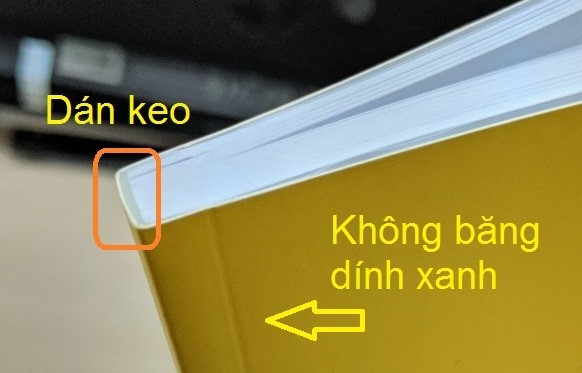
\includegraphics[scale=1]{figures/fig1}
		\caption{Dán keo}
		
		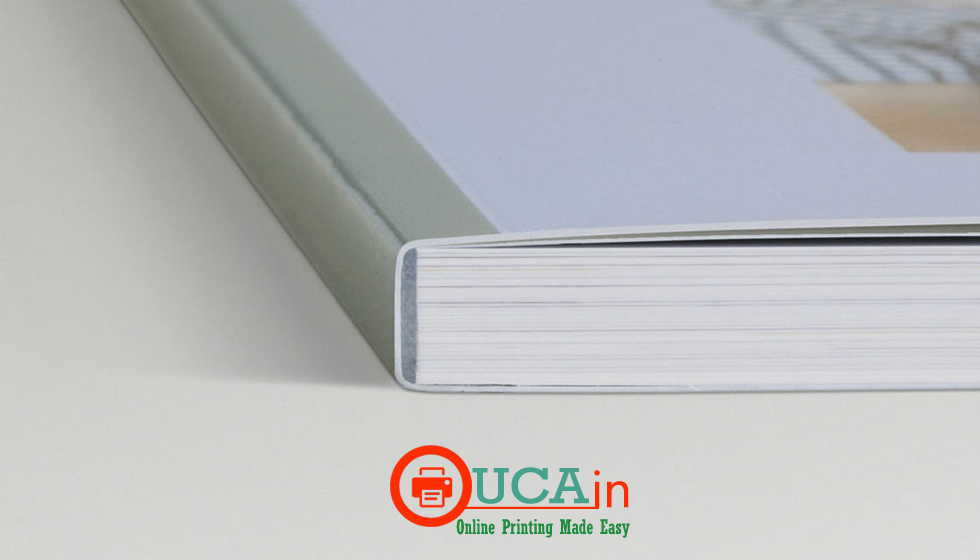
\includegraphics[scale=0.3]{figures/fig2}
		\caption{Không băng dính xanh}
	\end{figure}
	
Phần gáy ĐATN cần ghi các thông tin tóm tắt sau:
Kỳ~làm~ĐATN~-~Ngành~đào~tạo~-~Họ~và~tên~sinh~viên~-~Mã~số~sinh~viên.
\vspace{2cm}

Ví dụ:

\textbf{2019.1 - VẬT LÝ KỸ THUẬT - NGUYỄN VĂN A - 20141234}

Qui cách ghi chữ phần gáy như hình sau:

\begin{figure}
\centering
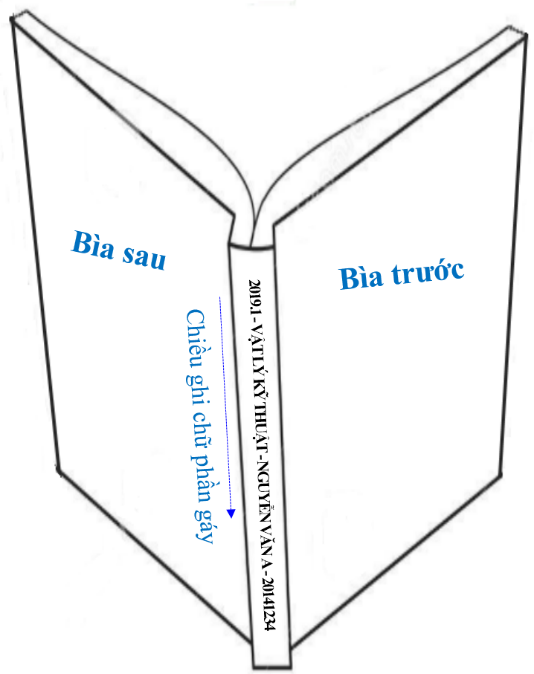
\includegraphics[scale=0.7]{figures/fig3}
\caption{Ghi chữ phần gáy}
\end{figure}


\chapter{SỬ DỤNG CÁC BIỂU ĐỒ}
\label{chap:bieudo}


\section{Giới thiệu về biểu diễn bằng đồ thị}
\label{sec:dothi}
Trong rất nhiều lĩnh vực cần phải trình bày, giới thiệu các thông tin liên quan tới con số, thống kê hay các dữ liệu khác. Các dữ liệu đo đạc, tính toán thường được thu thập dưới dạng bảng biểu; tuy nhiên bảng biểu chỉ thích hợp khi trình bày các số lượng nhỏ các số liệu, đồng thời không cung cấp các đánh giá trực quan về xu hướng của dữ liệu thu được.

Đồ thị có khả năng cung cấp hình ảnh trực quan, dễ hiểu giúp người đọc nhanh chóng nắm bắt được ý tưởng muốn nhấn mạnh, muốn trình bày. Người trình bày cần lựa chọn đúng loại đồ thị và không nên sử dụng các đồ thị quá màu mè; lựa chọn tên đồ thị ngắn gọn, dễ hiểu. Các loại đồ thị thường gặp là:
\begin{itemize}
	\item[-] Kiểu bánh (Pie charts)
	\item[-] Kiểu thanh ngang \& dọc (kiểu cột) (Horizontal \& Vertical bar charts)
	\item[-] Kiểu đường \& Kiểu phân bố (Line charts \& Scatter diagrams)
	\item[-] Kiểu diện tích (Area charts)
\end{itemize}

\begin{figure}[h]
\centering
	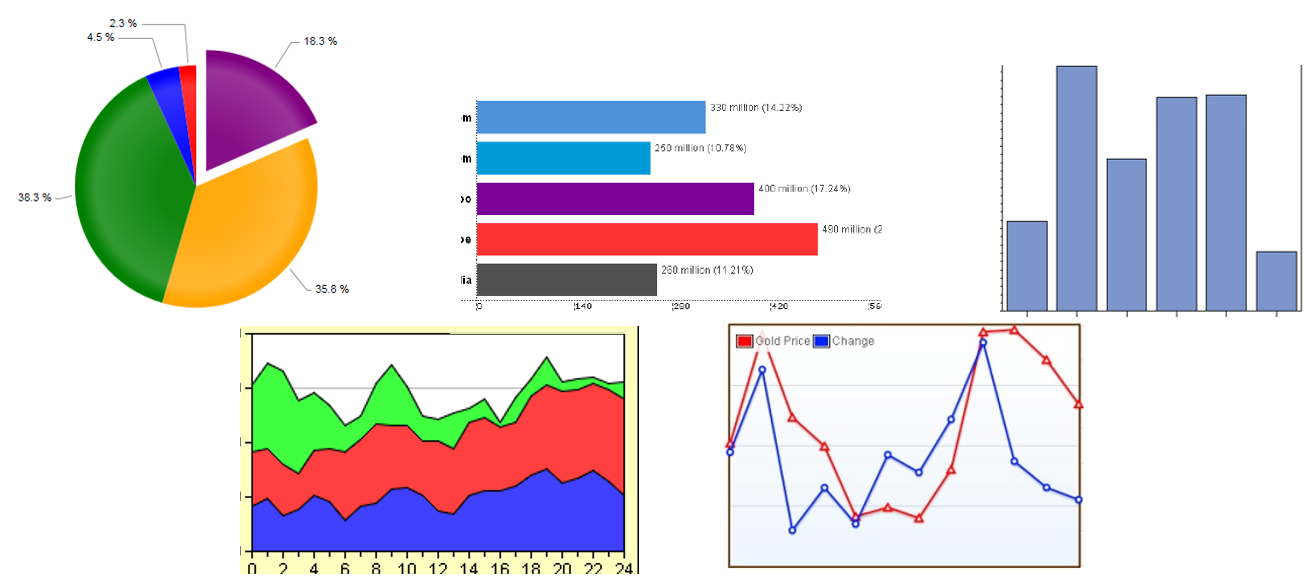
\includegraphics[scale=0.4]{figures/fig4}
\end{figure}

Phần tiếp theo sẽ khuyến cáo về phạm vi sử dụng của từng loại đồ thị này.
\section{Đồ thị kiểu bánh}
\label{sec:banh}
Phạm vi sử dụng:
\begin{itemize}
	\item[-] Dùng để biểu thị tỷ lệ phần trăm (\%)
	\item[-] Biểu diễn mối liên hệ tương quan tỷ lệ
	\item[-] Không nên dùng quá nhiều miếng (tối đa 6 miếng) trong một đồ thị
\end{itemize}
\begin{figure}[h]
\centering
	
\includegraphics[scale=0.5]{figures/fig5}
\end{figure}
Khi muốn nhấn mạnh một đại lượng:
\begin{itemize}
 \item[-] Để diễn tả phần quan trọng: đặt phần quan trọng này ở phía trên, bên phải, tính từ vị trí 1 giờ
 \item[-] Khi cần nhấn mạnh: có thể kéo phần nhô này ra khỏi đồ thị ( nhấn mạnh về tỷ trọng phần trăm của ngô là nhỏ nhất)
\end{itemize}

\begin{figure}[h]
\centering
	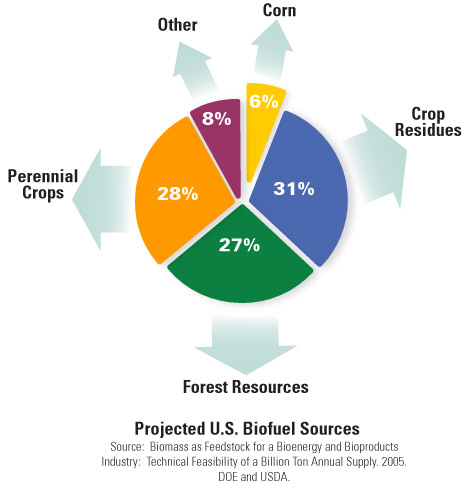
\includegraphics[scale=0.5]{figures/fig6}
\end{figure}

\section{Đồ thị kiểu thanh ngang}
\label{sec:thanhngang}

\section{Đồ thị kiểu cột đứng}
\label{sec:cotdung}

\section{Đồ thị kiểu diện tích}
\label{sec:dientich}

\chapter{KẾT LUẬN}
\label{chap:ketluan}

\section{Kết luận}
\label{sec:ketluan}
Nội dung phần kết luận này tùy thuộc vào từng đồ án. Lưu ý trong phần kết luận không nên có bất cứ phương trình, biểu đồ hay bảng biểu nào. Cần trình bày rõ nội dung đồ án tốt nghiệp đã đáp ứng đầy đủ các yêu cầu của đề bài hay chưa. Trình bày về ý nghĩa của các kết quả thu được, các đánh giá nhận xét về tính khả thi, tính chính xác của kết quả, tính thực tế của đồ án…Cần lưu ý hạn chế sử dụng các tính từ, trạng từ mạnh trong khi miêu tả kết quả đạt được, cần đảm bảo tính trung thực của các kết luận.

Trình bày các kiến thức mà sinh viên đã đạt được sau khi thực hiện đồ án tốt nghiệp. Đồng thời trình bày về các kỹ năng đã học được (kỹ năng tự tìm kiếm tài liệu, tổng hợp thông tin, kỹ năng chế bản, kỹ năng trình bày, viết báo….).

\section{Hướng phát triển của đồ án trong tương lai}
\label{sec:phattrien}
Nêu tóm tắt hướng mở rộng của đề tài trong tương lai nếu có. Đây là mục tùy chọn vì phụ thuộc vào loại đề tài.



\chapter{ch4}
\section{sec1}
\lipsum
\section{sec2}
\lipsum
\section{sec3}
\lipsum
\chapter{ch5}
\section{sec1}
\lipsum
\section{sec2}
\lipsum
\chapter{ch6}
\section{sec1}
\lipsum
\section{sec2}
\lipsum
\chapter{ch7}
\section{sec1}
\lipsum
\section{sec2}
\lipsum
\chapter{chương3}
\section{sec2}
\lipsum
\section{sec2}
\lipsum
\chapter{chương2}
\lipsum
\chapter*{chương3}
\lipsum

Tiep Vu \textit{et. al.}\cite{knuthwebsite,vu2016histopathological}
Thức Trần \cite{einstein,vu2015dfdl}
\bibliographystyle{IEEEtran}
\bibliography{literature/refs}

\end{document}